\documentclass[midd]{thesis}

\usepackage{graphicx}
\usepackage{times}
\usepackage{amsmath}

\bibliographystyle{plain}


\title {Computational Aesthetic Evaluation using Convolutional Neural Networks: Hard Lessons Learned with Machine Learning}

\author {Teddy Knox}
\adviser {Professor Christopher Andrews}

\begin{document}

\maketitle

\begin{abstract}
The accuracies of state-of-the-art machine learning techniques have exceeded the accuracy of humans at certain limited tasks, suggesting the computers will soon be able to complete many sophisticated tasks competently. This study tested the accuracy of state-of-the-art convolutional neural networks for modeling the statistically-defined visual aesthetic tastes of an individual. Our trained model achieved 74\% accuracy in distinguishing aesthetically pleasing and displeasing abstract generative art, suggesting that deep learning techniques may be well-suited to the task of modeling the statistical distribution of arbitrary user tastes.
\end{abstract}

\begin{acknowledgements}
I dedicate this paper to science.
\end{acknowledgements}

\contentspage
\tablelistpage
\figurelistpage

\normalspacing \setcounter{page}{1} \pagenumbering{arabic}

\chapter{Introduction}
\label{sec:intro}

Machine learing is a broad discipline of computer science that has seen rapid advances in recent years, and has the potential to impact all human enterprises. The latest algorithms are capable of competitive or even better-than-human performance [citation needed] on certain tasks, and their applications are increasing in proportion to the availability of training data. One such application will be in the more  field of generative art and design. Generative art is art that is created procedurally, often with the help of a computer. Until recently, the use of computers in art and design has been limited to rote tasks such as preparing renderings and generating randomness, but advances in machine learning may soon lend computers to more high-level aspects the creative process, such as creative exploration and Computational Aesthetic Evaluation. Computation Aesthetic Evaluation (CAE) is the problem in generative art research of programming a computer to subjectively differentiate between aesthetically pleasing and displeasing content. This problem is important to the field of generative art for its potential to automate searches for aesthetic solutions, and would also be useful for building personalized recommendation systems. This research investigates the applicability of state-of-the-art general-purpose pattern recognition algorithms for Computational Aesthetic Evaluation. This experimentation is motivated by an interest in discovering the limits of these impressive models. By evaluating their accuracy on unconventional datasets of unknown complexity, we hope to gain a better understanding of both the model's capabilities and the hidden structure of the dataset. This paper first provides background and formulates the problem, then explains the experimentation in detail, and concludes with a discussion of results and future uses of machine learning models for the analysis of artistic content.

% general introduction to CAE and generative art
% why we would care? vision
% WHat is this particular thesis about -> applying ml to the problem
% what are we doing? -> convolutional neural network
% more specific -> ran a study, using GoogLeNet
% What we will discuss ->

Convolutional Neural Networks (CNNs) are a type of model inspired by the biology of the human visual processing center, and have been shown to be the most effective model for image recognition to date. CNNs are a type of feed-forward artificial neural network architecture formed by layers of are convolutional filters, trained to derive high-level features from low-level pixel data. These high-level features are powerful and versatitle differentiators of the training data, and are typically fed into a non-linear classifier or regressor to produce final predictions. The network's parameters are learned through an iterative training process, where batches of examples are fed into the network and network parameters are adjusted to reduce prediction errors. Iterations of adjustments are made until the network's prediction accuracy on its training data converges or surpasses a threshold. The CNN training process is computationally intentensive, with a requiring training time that grows quickly with the width and depth of layers. The main model we used for classification is a replica of the Google Research entry into the 2014 Imagenet Large-Scale Visual Recognition Challenge (ILSVRC 2014), dubbed GoogLeNet. Imagenet is an image database organized according to the wordnet hierarchy, and the ILSVRC 2014 challenge tested the ability of models to accurately tag photos with up to 5 tags out of a body of 1000. The GoogLeNet architecture won the ILSVRC challenge in 2014, achieving an impressive top-5 error rate of 6.67\%. GoogLeNet is an extremely deep network comprised of 24 layers, [how many convolutional layers?], and operates with [how many parameters?]. A full discussion of the qualities and mechanics of convolutional neural networks will come in the theory section.

Accurate Computational Aesthetic Evaluation algorithms would be useful in the fields of generative art and recommendation systems. With the invention of modern computers, the limiting factor on the increasing prevalance and complexity of generative art has become the artist, specifically their expertise in creative decision making and aesthetic evaluation. Despite their enormous computational power, the primary use of modern computers in generative art falls into the category of rendering procedures into their realized form, rather than participating in the search for aesthetic beauty. Advances in machine learning for pattern recognition have proved useful in many different types of well-defined tasks. In this study we apply modern image classification techniques using convolutional neural networks to the problem of computational aesthetic evaluation, observing whether they are capable of learning the tastes evident in a dataset of randomly generated triangle art, labeled with aesthetic quality ratings.

% Discussion of how art school guidelines are products of aesthetics but are too reductive to explain the underlying phenomena. Can only confirm theories.
  % In other words, the supervised techniques capable of recognizing a dog in an image may also be effective at recognizing a well-composed photograph. This presupposes Several difficult modeling tasks could soon be easier thanks to these advances
  % The task of computational aesthetic evaluation (CAE) is to judge the aesthetic value of a piece of artwork according to subjective criteria. The most groundbreaking advances on this task will likely stem from insights into the neural heuristics underpinning near-universal human preference for qualities such as consonance and composition, leading to new unsupervised learning techniques. Although these techniques will lay a foundation for more naturaly.
  % expand on this
  % - biological inspiration, history
  % - rough explanation of using lower level features to construct higher level features
  % - introduction of GoogLeNet
  % Google - a computer can do anything a human can do in under a second
  % does not take into account aspects of novelty
    % Two ways to go:
    % - Computational Aesthetic Evaluation
    % - Recommendation systems
  % Convolutional neural networks and the nature of training sets and computational aesthetic evaluation
  % - Not as much work in computer imagined art -- art which presents a few layers of abstraction so that each result is
  % unique and valuable on its own
  % - The goal, of course, when it comes to art is to produce beauty. But this in itself is not a simple concept.
  %   The branch of philosophy called Aesthetics can lend us some insight into where to look for answers.
  % - sensory tastes vary from person to person, although beauty is different as it is generally claimed as a universal
  %   property of a thing.
  % - Emanuel Kant argued that judgements of beauty are sensory, emotional and intellectual all at once,
  %   as opposed to judgements of enjoyment which are purely sensory.
  % - Contemporary views on beauty refuse such a thing as universal beauty, attributing such aesthetic certainties to the
  %   power of culture to shape opinions similarly.
  % - At the same time, it's fairly likely that humans have an innate disposition for certain aesthetics
  %   - think musical consonance and disonance
  %   - or facial or physical beauty for sexual reproduction (along with facial expressions)
  %   - Some have theorized that aesthetic pleasure has to do with the resolution of apparent complexity into compressed
  %     representations.
  %     - If so, might it be possible to train a classifier to recognize these complex compositions
  %       with compact representations.
  % - We experiment with state-of the art Convolutional Neural Networks to predict the subjective aesthetic beauty.

\chapter{Related Work}

Computational Aesthetics is a burgeoning interdisciplinary field that aims to develop systems for assesing the aesthetic value of art, music, or design. As an interdisciplinary field, many of the its advances have stemmed from the synthesis of advances in the respective fields of machine learning, neuroaesthetics, and philosophy.

Aesthetics represent one of the oldest fields of philosophy, but only recently has any formal unifying theory gained traction. One of the most significant advances in aesthetics is owed to Mathematician G.D. Birkoff, who spent a year traveling the world to beauty across cultures, before proposing a speculative psychological model for quantifying it. In his oft-referenced 1933 paper \emph{Aesthetic Measure}, Birkoff proposes that the perception of beauty as the pleasurable resolution of apparent complexity of a stimulus into a compact mental representation. He codified this relationship into a formula that relates degree of beauty $B$ to the balanced ratio of order $O$ to complexity $C$.

\begin{align*}
B &= \frac{C}{O}
\end{align*}

The plausibility of Birkoff's measure as a guiding philosophy of aesthetics earned it significant attention in later experimental studies. The recent work of Ragau et. al. and Koshel et. al. draws from information theory to approximate the parameters of Birkoff's formula. They used zeroth-order measures such as Kolmogorov complexity and Shannon entropy \cite{rigau-1, koshelev-1}, to demonstrate encouraging correlations between Birkoff's measure and human-rated beauty.

These results are significant enough to validate the direction Birkoff's core idea --- that the human aesthetic response is tuned to respond to stimuli that are sophisticated yet digestable. Novel ideas in the fields of machine learning, neuroaesthetics (the study of aesthetics from a biological perspective), and the emerging field of evolutionary philosophy (The top-down study of evolutionary adaptations), may be a way forward. Scientist Philip Galanter stands at the intersection of these fields, and subscribes to the view that humans find stimuli with the greatest ``effective complexity'' to be the most engaging, and thus the most rewarding. Within this framework, the problem of computational aesthetics can be expressed as the study of how humans judge ``effective complexity'' \cite{galanter-1,galanter-2,galanter-3,galanter-4}. Effective complexity is a theoretical measure conceived by Gell-Man et. al. \cite{gell2004effective} to roughly correspond to the colloquial meaning of the word ``complex''. Effective complexity meausures resistance to entropic forces rather than resistance to signal compression. For example, a symphony by Mozart possesses greater effective complexity than white noise, because it presents a manageable amount of harmonious sophistication for us to process.

\begin{figure}
\centering
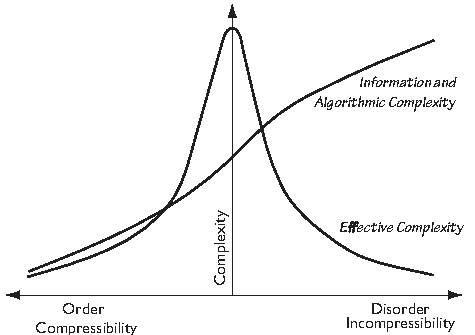
\includegraphics[width=0.75\textwidth]{figures/effectivecomplexity.pdf}
\caption{Relationship between effective complexity and order}
\label{fig:effectivecomplexity}
\end{figure}

In seeking to develop a computational aesthetic evaluator this reseach is touching onto topics of information complexity and effective complexity, as developed by these researchers. These improving measures will likely align closely with the neurology of human sensory perception. It may already be possible to draw parallels between the principles underlying machine learning systems and Birkoff's measure, since the success of these systems already depend on learning of compact, high-level represenations of low-level inputs. This is one of the reasons we became interested in applying the latest advances in image recognition to the field of computational aesthetics. Convolutional neural networks are models inspired by the structure of the human visual cortex, and as such may have a higher chance of making accurate predictions.

Several types of machine learning techniques have been used in computational aesthetic evaluation algorithms with increasing success. Penousal Machado et al \cite{machado2008experiments} implemented an iterative artificial artist system by combining a neural network with an evolutionary programming system. The neural network served as aesthetic evaluator, and was trained on manually extracted features for every step of the iteration. The genetic programming system would generate populations of artwork, using the aesthetic evaulator as its fitness function. In observing the creative process as alternation between creative and evaluative stages, their system repeatedly produces populations of ``drafts'' and then evaluates how well they match a constant set of target images. The target images they chose were pieces of artwork. The drafts that most closely matched the target images would then seed the next generation of drafts, and the aesthetic evaluator would be retrained to recognize all of the drafts as non-target images. This feedback loop was designed to ensure that every generation of drafts is different from the last, and hopefully resulting in greater image complexity. The entire algorithm produces interesting results until the 12th generation, when classification error increases steeply. The system's aesthetic evaluator uses 41 features based metrics like fractal complexity and zipf distribution, each applied over a variety of image channels such as hue or saturation. Even as more evolved drafts are added to the non-target training set, the classifier consistently trains to more than 99\% accuracy. This is to say that when asked to differentiate between images of paintings and computer generated images of previous generations, the classifier is accurate. The accuracy of the classifier on the next generation of drafts is much less stable. As the system's iterations progress, the neural network's accuracy for classifying the next generation of drafts based on previous generations steadily decreases, and then drops around iteration 12.


- their feature extractor is weak

Talk about other experiements to recognize aesthetics using Neural Networks.

Talk about applications of CAEs for Intelligent Interactive systems, Recommendation systems (as opposed to collaborative filtering), or Artificial Artistry. Cite some papers for each.

- Several others have applied genetic algorithms to optimize heuristics for aesthetic quality. For instance, a group
- seeking to automatically generate layouts for page content used the heuristic of minimizing wasted space as a fitness function on their population of layouts.

\section{Related Work in Image Classification}

Machine learning undergoes waves of research followed by recessions following collapsed hype. Currently we are undergoing a boom in machine learning research progress.

A list of the lead researchers Hinton, LeCunn, Google research, ...

- Going deeper with convolutions
- Paper that lead to Caffe

\chapter{Theory}

Deeper discussion on color theory generalizations.

\section{Generative Art}

Three factors went into the selection of the type of artwork to be used in this experiment. First, a body of art with a significant variance in subjective quality was desirable, since the experiment hinges on judging differences in quality. Next, a type of art with sufficiently simple characteristics was desirable to make the job of image classification as simple as possible without sacrificing the fundamental complexities of color scheme and composition. Last, in order to collect a large corpus of images quickly, an artform allowing for an efficient curation process was desirable. A corpus generative art lends itself nicely to these three constraints, since the randomness inherent tends to result in a variance in quality, the sophisitcation of abstract art is relatively low, and an endless pool of images can be sourced instantaneously.

I designed an extremely simple generative art method for producing our corpus of data. To produce an image, the program randomly places a random number of randomly-colored triangles on a randomly-colored background. I used a uniform random distribution in every case. I bounded the possible number of triangles, and limited the lightness of colors to a range, to boost the ratio of good results to bad results.

\section{Compuational Aesthetic Evaluation - Convolutional Neural Network}

We will use various CNN models that come with Caffe \"out of the box\" to test their efficacy, rather than attempt to customize a model to this task. The first model we will test is called GoogLeNet, which won the ImageNet Large Scale Visual Recognition Challenge in 2014.

\chapter{Implementation}

\section{Generative Art}

I designed a web interface for recording a binary rating to 4000 generated images, each three times, to form a composite score for each image. At each training interval, the trainer is shown an image on the screen, and asked to rate its quality as \"good\" or \"bad\". Sometimes the trainer is shown an image they have rated before, in order to corroborate the quality of the image.

The business logic of this training interface is written in python, because Caffe supports python bindings to its functionality. The images were drawn using the \"pillow\" python package. I opted not to use processing because I was unaware of any processing port to python.

% - Once we have a functioning model, we plan use it in the generation of new images to filter out bad random results.

\section{Compuational Aesthetic Evaluation - Convolutional Neural Network}

I chose to use the Caffe framework for image recognition for its documentation and widespread adoption in the machine learning community.

We will train GoogLeNet on a random subset of the images, and test it on the rest.

\chapter{Results}

I put together a training corpus of 4000 images, each with 3 binary ratings.

I plan to use standard metrics for measuring the effectiveness of our classifier.

I plan to use our model to filter ugly results from our triangle art generator and showcase the quality of the CAE model on free range images.

If time allows, I plan to feed different classes of artwork into the CAE model to test its efficacy at applying aesthetic preferences learned with the abstract shapes to forms of higher complexity.

\chapter{Conclusion}

Given the difficulty of defining art itself, it is no surprise that the criticism and reception of art itself is as nebulous. Yet despite the unclear underpinnings of aesthetic tastes, it is clear that aesthetic judgements are an integral part of everyday life. Short of machine intelligence, computerized judgements of aesthetics will likely never supercede our own, but in combination with our own, there is the potential for computers to make artists out of us all, or at least reduce the cost of aesthetically pleasing design.

The outcome of this experiment may not be clear and but the field of computational aesthetic evaluation will only gain in relevance as we strive to make our world more beautiful.

% - Is there a unifying aspect behind the beauty of various types of things?
% - Could we teach a computer to find a beautiful solution to a problem by studying how to generate beautiful artwork?
% - There have been much academic discussion of questions of where to begin with the problem of Computation Aesthetic Evaluation.
% - the general consesnus is: baby steps.
% - A deeply interconnected problem
%   - why?

Qualitative results here

\nocite{*}
\bibliography{thesis}
\end{document}

%% LaTeX Examples

% This thesis has many chapters.  For more on Alice see
% Chapter~\ref{sec:alice}, and in particular Section~\ref{sec:reproach}.
%% \section{SECTION 1}
% The text for Section 1 goes here.
% \label{sec:alice}
% \subsection{Subsection heading goes here}
% Subsection 1 text
% \subsubsection{Subsubsection 2 heading goes here}
% Subsubsection 2 text
% \begin{equation}
% \label{eqn:sampleEqn}
% k_1=\frac{\omega }{c({1/\varepsilon_m + 1/\varepsilon_i})^{1/2}}=k_2=\frac{\omega
% sin(\theta)\varepsilon_{air}^{1/2}}{c}
% \end{equation}
%
% \noindent
% where $\omega$ is the frequency of the plasmon, $c$ is the speed of
% light, $\varepsilon_m$ is the dielectric constant of the metal,
% $\varepsilon_i$ is the dielectric constant of neighboring insulator,
% and $\varepsilon_{air}$ is the dielectric constant of air.
% Equation~\ref{eqn:sampleEqn} makes this perfectly clear.
% See also Figure~\ref{fig:myfig} for an illustration.
%
%
% \begin{figure}
% \centering
% 
\includegraphics[width=0.75\textwidth]{graph.png}
% \caption{My figure.}
% \label{fig:myfig}
% \end{figure}
%%
% (As promised in Chapter~\ref{sec:intro}, here it gets interesting.)
%
% \appendix
% \chapter{Chapter 1 of appendix}
% Appendix chapter 1 text goes here
